% Options for packages loaded elsewhere
\PassOptionsToPackage{unicode}{hyperref}
\PassOptionsToPackage{hyphens}{url}
%
\documentclass[
]{article}
\usepackage{amsmath,amssymb}
\usepackage{iftex}
\ifPDFTeX
  \usepackage[T1]{fontenc}
  \usepackage[utf8]{inputenc}
  \usepackage{textcomp} % provide euro and other symbols
\else % if luatex or xetex
  \usepackage{unicode-math} % this also loads fontspec
  \defaultfontfeatures{Scale=MatchLowercase}
  \defaultfontfeatures[\rmfamily]{Ligatures=TeX,Scale=1}
\fi
\usepackage{lmodern}
\ifPDFTeX\else
  % xetex/luatex font selection
\fi
% Use upquote if available, for straight quotes in verbatim environments
\IfFileExists{upquote.sty}{\usepackage{upquote}}{}
\IfFileExists{microtype.sty}{% use microtype if available
  \usepackage[]{microtype}
  \UseMicrotypeSet[protrusion]{basicmath} % disable protrusion for tt fonts
}{}
\makeatletter
\@ifundefined{KOMAClassName}{% if non-KOMA class
  \IfFileExists{parskip.sty}{%
    \usepackage{parskip}
  }{% else
    \setlength{\parindent}{0pt}
    \setlength{\parskip}{6pt plus 2pt minus 1pt}}
}{% if KOMA class
  \KOMAoptions{parskip=half}}
\makeatother
\usepackage{xcolor}
\usepackage{graphicx}
\makeatletter
\def\maxwidth{\ifdim\Gin@nat@width>\linewidth\linewidth\else\Gin@nat@width\fi}
\def\maxheight{\ifdim\Gin@nat@height>\textheight\textheight\else\Gin@nat@height\fi}
\makeatother
% Scale images if necessary, so that they will not overflow the page
% margins by default, and it is still possible to overwrite the defaults
% using explicit options in \includegraphics[width, height, ...]{}
\setkeys{Gin}{width=\maxwidth,height=\maxheight,keepaspectratio}
% Set default figure placement to htbp
\makeatletter
\def\fps@figure{htbp}
\makeatother
\setlength{\emergencystretch}{3em} % prevent overfull lines
\providecommand{\tightlist}{%
  \setlength{\itemsep}{0pt}\setlength{\parskip}{0pt}}
\setcounter{secnumdepth}{-\maxdimen} % remove section numbering
\ifLuaTeX
  \usepackage{selnolig}  % disable illegal ligatures
\fi
\usepackage{bookmark}
\IfFileExists{xurl.sty}{\usepackage{xurl}}{} % add URL line breaks if available
\urlstyle{same}
\hypersetup{
  pdftitle={RCTab: An Azure Subscription Management System},
  hidelinks,
  pdfcreator={LaTeX via pandoc}}

\title{RCTab: An Azure Subscription Management System}
\author{}
\date{29 April 2024}

\begin{document}
\maketitle

\subsection{Summary}\label{summary}

The advent of commercial cloud services has provided researchers with
the benefits of flexible and scalable computing and storage resources.
However, cloud providers do not always provide cost control measures
with ability to enforce strict budget controls, potentially allowing
users to overspend. This presents serious challenges for adoption in
research organisations that need to centrally disseminate cloud
resources to researchers with independent budgets. In response, we have
developed \href{https://rctab.readthedocs.io/}{RCTab} (\textbf{R}esearch
\textbf{C}omputing \textbf{Tab}les), an open-source system for budget
control and
\href{https://learn.microsoft.com/en-us/azure/cloud-adoption-framework/ready/azure-setup-guide/organize-resources\#management-levels-and-hierarchy}{subscription}
management on Azure, Microsoft's cloud computing platform. RCTab enables
organisations to centrally manage cloud resources while enforcing strict
budget controls. Organisations can allocate budgets, and RCTab will
automatically monitor usage and shut down cloud resources when it is
consumed. It enables users to monitor their budget usage via a web
interface and email alert system. RCTab is designed to be customisable
and extensible, so can be easily adapted to the needs of different
organisations. It is written in Python and has Infrastructure as Code
(IaC) deployment for quick and reliable deployment to Azure.

\subsection{Statement of Need}\label{statement-of-need}

Institutions are adopting cloud platforms, such as Amazon Web Services,
Microsoft Azure and Google Cloud Platform, for their operational and
research computing infrastructure. However, on-demand
pricing\footnote{With ``on-demand'' or ``pay as you go'' pricing,
  customers are billed for what they use, with no upfront costs.
  Although it is not the only cloud pricing option, it is the simplest
  and the most common.}, can present challenges for organisations that
require certainty in their expenditure.

This is especially true for organisations with technical users, who
require both autonomy and access to the latest hardware, such as
multi-GPU virtual machines. The limitations of budget monitoring and
enforcing tools can require organisations to either limit the number of
users accessing resources and the type of resources they can access or
employ dedicated staff to monitor resource usage and costs. Neither
approach is ideal: the former can restrict the cloud's potential, while
the latter is time-consuming and error-prone.

Microsoft Azure, which is the focus of this work, offers tools for
managing costs, such as budgets, cost alerts, and cost analysis\cite{azurecm}.
These tools are designed for individual subscriptions, and
they do not scale effectively for organisations with many subscriptions.
Moreover, they do not offer a mechanism to impose strict limits on
spending, instead sending alerts when the threshold is exceeded, or
specify the duration for which a budget is valid.

Our response to this challenge is the development of
\href{https://rctab.readthedocs.io/}{RCTab}, an open-source system for
automating the management of subscriptions on Azure.

RCTab has been developed by the Alan Turing Institute's Research
Computing team and is used at the Institute to oversee hundreds of
subscriptions used by researchers and support staff with plans to expand
its use to other organisations and cloud providers.

\subsection{Codebase}\label{codebase}

The source code for RCTab is contained in five repositories:

\begin{itemize}
\tightlist
\item
  the \href{https://github.com/alan-turing-institute/rctab-cli}{CLI}
  repository contains the command-line interface (used for
  administrative tasks), which is a Pip-installable Python package.
\item
  the
  \href{https://github.com/alan-turing-institute/rctab-infrastructure}{Infrastructure}
  repository contains code for automated deployment with
  \href{https://www.pulumi.com/}{Pulumi}.
\item
  the \href{https://github.com/alan-turing-institute/rctab-api}{API}
  repository has code for the webserver, which is pushed
  \href{https://hub.docker.com/r/turingrc/rctab-api}{to DockerHub} each
  time there is a new release.
\item
  the
  \href{https://github.com/alan-turing-institute/rctab-functions}{Functions}
  repository contains three Azure function apps, which are also pushed
  to DockerHub
  (\href{https://hub.docker.com/r/turingrc/rctab-usage}{usage},
  \href{https://hub.docker.com/r/turingrc/rctab-status}{status} and
  \href{https://hub.docker.com/r/turingrc/rctab-controller}{controller})
  each release.
\item
  the \href{https://github.com/alan-turing-institute/rctab}{eponymous
  repository} houses the general documentation (the other repositories
  also have sites for component-specific documentation).
\end{itemize}

Detailed instructions on how to deploy RCTab to Azure with Pulumi can be
found in the docs for the
\href{https://github.com/alan-turing-institute/rctab-infrastructure}{Infrastructure}
repository. Once Pulumi has been installed and the necessary settings
have been configured, an instance of RCTab can be deployed or destroyed
in minutes. Additional instances (e.g.~for testing) can also be created
quickly.

\subsection{Operation}\label{operation}

Once deployed to Azure, an instance of RCTab will comprise:

\begin{itemize}
\tightlist
\item
  A FastAPI web server, which uses the API Docker image. This allows
  users to view budgets, Role-Based Access Control (RBAC) assignments
  and the state of subscriptions.
\item
  Three function apps, running their respective Docker images, that
  collect data and enable/disable subscriptions.
\item
  A PostgreSQL database.
\item
  Logging and alerts.
\end{itemize}

\begin{figure}
\centering
\includegraphics{figure1.png}
\caption{System diagram.\label{fig:Figure 1}}
\end{figure}

Users can use the web frontend to see subscriptions' spending and budget
details, such as remaining amount, expiration date, the project to which
spending will be charged and list of RBAC assignments.

Administrators can use the CLI to create and edit budgets, override
budgets (for critical subscriptions that must never be turned off) and
get summaries.

RCTab integrates with Microsoft Entra ID (previously ``Azure Active
Directory'') to provide ``Single Sign On'' authentication for the
frontend and CLI.

The Usage and Status functions run on a schedule to collect information
about subscriptions' recent spending and current state, respectively,
and post it to the web server.

The Controller function will poll the web server to see whether any
subscriptions need to be turned off or on.

The web server will email users about changes to their subscriptions and
send daily email summaries to administrators.

\subsection{Lifecycle of a
Subscription}\label{lifecycle-of-a-subscription}

A simple method for organising an Azure tenant is to create one
subscription per project (or per-group or per-department, etc). RBAC
assignments can be used to grant permissions to researchers at the
subscription level, giving them the freedom to create, modify and delete
resources within that subscription as their work requires.

Once a subscription has been created, it will need to be placed into a
management group visible to RCTab. RCTab will manage those subscriptions
it has read/write access to and monitor those that it has read-only
access to.

\begin{figure}
\centering
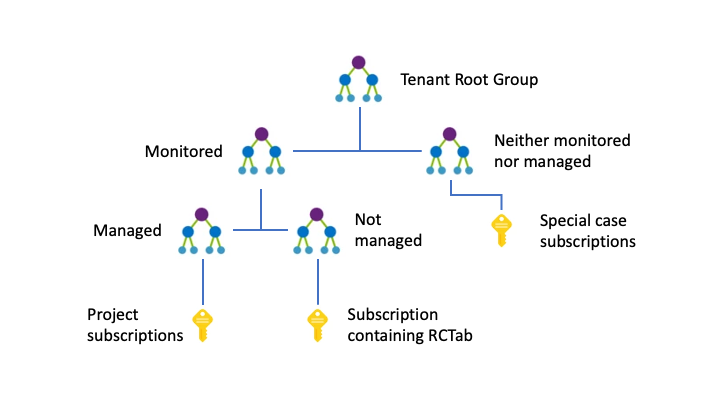
\includegraphics{figure2.png}
\caption{Management group hierarchy.\label{fig:Figure 2}}
\end{figure}

Using the CLI, an administrator can add an ``approval'' for the
subscription to RCTab that specifies the amount and duration of the
budget for the subscription.

When the subscription approaches its budget or expiration date, RCTab
will email users with role assignments to give them a chance to request
a budget increase or an extension.

If this is granted, the admin can extend the approval with the CLI. The
approval has fields to link to the email or support request used to
request the extension.

If the request is denied, the subscription will be disabled by RCTab
and, again, users will be notified by email. Azure will permanently
delete the subscription after approximately 90 days, though the
subscription can be re-activated up until that point.

\subsection{Acknowledgements}\label{acknowledgements}

\begin{itemize}
\tightlist
\item
  This work was supported in part through computational resources
  provided by The Alan Turing Institute under EPSRC grant EP/N510129/1
  and with the help of a generous gift from Microsoft Corporation.
\item
  Oscar Giles is the original project author, responsible for the
  initial design and implementation of the API and CLI.
\item
  Iain Stenson added the function apps and newer features of the API and
  CLI.
\item
  Tomas Lazauskas provided guidance and support for the project, as well
  as contributions to the API codebase.
\item
  Joseph Palmer refined the automated deployment and the front-end
  details pages, amongst other work.
\item
  Pamela Wochner added summary emails, as well as work on preparations
  for making the project open-source.
\item
  In addition to code review and contributions, Eseoghene Ben-Iwhiwhu
  provided feedback on the documentation.
\item
  We would like to acknowledge code and documentation contributions by
  Markus Hauru, Jim Madge and Federico Nanni.
\end{itemize}
\begin{thebibliography}{9}

\bibitem{azurecm}
    Cost management documentation,
    Azure,
    https://learn.microsoft.com/en-us/azure/cost-management-billing/costs/,
    Accessed 29 April 2024. 

\end{thebibliography}
\end{document}
